\documentclass{standalone}
\usepackage{tikz}
\usetikzlibrary{patterns, positioning}


\begin{document}
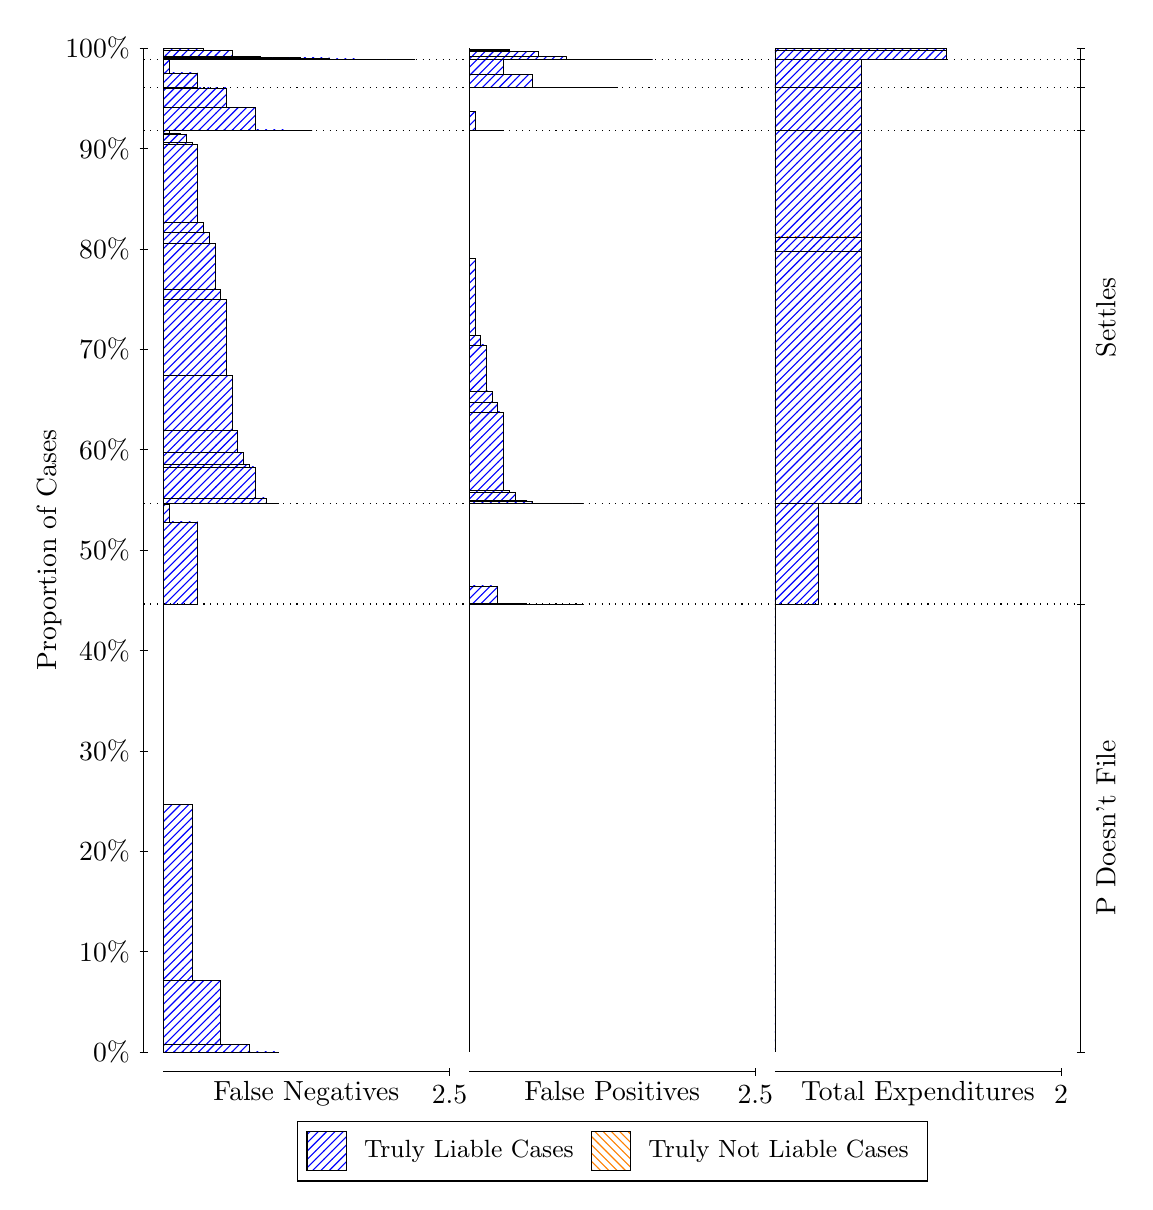
\begin{tikzpicture}
\draw[black, very thin] (1.5,1.75) -- (1.5,14.5);
\node[rotate=90, text=black, anchor=center] at (0.3, 8.125) {Proportion of Cases};
\draw[black, very thin] (1.45,1.75) -- (1.55,1.75);
\node[text=black, anchor=east] at (1.45, 1.75) {0\%};
\draw[black, very thin] (1.45,3.025) -- (1.55,3.025);
\node[text=black, anchor=east] at (1.45, 3.025) {10\%};
\draw[black, very thin] (1.45,4.3) -- (1.55,4.3);
\node[text=black, anchor=east] at (1.45, 4.3) {20\%};
\draw[black, very thin] (1.45,5.575) -- (1.55,5.575);
\node[text=black, anchor=east] at (1.45, 5.575) {30\%};
\draw[black, very thin] (1.45,6.85) -- (1.55,6.85);
\node[text=black, anchor=east] at (1.45, 6.85) {40\%};
\draw[black, very thin] (1.45,8.125) -- (1.55,8.125);
\node[text=black, anchor=east] at (1.45, 8.125) {50\%};
\draw[black, very thin] (1.45,9.4) -- (1.55,9.4);
\node[text=black, anchor=east] at (1.45, 9.4) {60\%};
\draw[black, very thin] (1.45,10.675) -- (1.55,10.675);
\node[text=black, anchor=east] at (1.45, 10.675) {70\%};
\draw[black, very thin] (1.45,11.95) -- (1.55,11.95);
\node[text=black, anchor=east] at (1.45, 11.95) {80\%};
\draw[black, very thin] (1.45,13.225) -- (1.55,13.225);
\node[text=black, anchor=east] at (1.45, 13.225) {90\%};
\draw[black, very thin] (1.45,14.5) -- (1.55,14.5);
\node[text=black, anchor=east] at (1.45, 14.5) {100\%};

\draw[black, very thin] (13.4,1.75) -- (13.4,14.5);
\draw[black, very thin] (13.35,1.75) -- (13.45,1.75);
\node[anchor=west] at (13.35, 1.75) {};
\draw[black, very thin] (13.35,7.4391) -- (13.45,7.4391);
\node[anchor=west] at (13.35, 7.4391) {};
\draw[black, very thin] (13.35,8.7133) -- (13.45,8.7133);
\node[anchor=west] at (13.35, 8.7133) {};
\draw[black, very thin] (13.35,13.452) -- (13.45,13.452);
\node[anchor=west] at (13.35, 13.452) {};
\draw[black, very thin] (13.35,13.997) -- (13.45,13.997);
\node[anchor=west] at (13.35, 13.997) {};
\draw[black, very thin] (13.35,14.357) -- (13.45,14.357);
\node[anchor=west] at (13.35, 14.357) {};
\draw[black, very thin] (13.35,14.5) -- (13.45,14.5);
\node[anchor=west] at (13.35, 14.5) {};

\draw[black, very thin, pattern color=blue, pattern=north east lines] (1.75,1.75) rectangle (3.2033,1.7509);
\draw[black, very thin, pattern color=blue, pattern=north east lines] (1.75,1.7509) rectangle (2.84,1.8473);
\draw[black, very thin, pattern color=blue, pattern=north east lines] (1.75,1.8473) rectangle (2.4767,2.6545);
\draw[black, very thin, pattern color=blue, pattern=north east lines] (1.75,2.6545) rectangle (2.1133,4.8923);
\draw[black, very thin, pattern color=orange, pattern=north west lines] (1.75,4.8923) rectangle (1.75,4.8923);
\draw[black, very thin, pattern color=blue, pattern=north east lines] (1.75,4.8923) rectangle (1.75,7.4391);
\draw[black, very thin, pattern color=blue, pattern=north east lines] (1.75,7.4391) rectangle (2.186,8.4827);
\draw[black, very thin, pattern color=blue, pattern=north east lines] (1.75,8.4827) rectangle (1.8227,8.7071);
\draw[black, very thin, pattern color=orange, pattern=north west lines] (1.75,8.7071) rectangle (1.75,8.7071);
\draw[black, very thin, pattern color=blue, pattern=north east lines] (1.75,8.7071) rectangle (1.75,8.7133);
\draw[black, very thin, pattern color=blue, pattern=north east lines] (1.75,8.7133) rectangle (3.2033,8.7134);
\draw[black, very thin, pattern color=blue, pattern=north east lines] (1.75,8.7134) rectangle (3.058,8.7868);
\draw[black, very thin, pattern color=blue, pattern=north east lines] (1.75,8.7868) rectangle (2.9127,9.1804);
\draw[black, very thin, pattern color=blue, pattern=north east lines] (1.75,9.1804) rectangle (2.84,9.2117);
\draw[black, very thin, pattern color=blue, pattern=north east lines] (1.75,9.2117) rectangle (2.7673,9.3685);
\draw[black, very thin, pattern color=blue, pattern=north east lines] (1.75,9.3685) rectangle (2.6947,9.6485);
\draw[black, very thin, pattern color=blue, pattern=north east lines] (1.75,9.6485) rectangle (2.622,10.34);
\draw[black, very thin, pattern color=blue, pattern=north east lines] (1.75,10.34) rectangle (2.5493,11.311);
\draw[black, very thin, pattern color=blue, pattern=north east lines] (1.75,11.311) rectangle (2.4767,11.434);
\draw[black, very thin, pattern color=blue, pattern=north east lines] (1.75,11.434) rectangle (2.404,12.018);
\draw[black, very thin, pattern color=blue, pattern=north east lines] (1.75,12.018) rectangle (2.3313,12.163);
\draw[black, very thin, pattern color=blue, pattern=north east lines] (1.75,12.163) rectangle (2.2587,12.286);
\draw[black, very thin, pattern color=blue, pattern=north east lines] (1.75,12.286) rectangle (2.186,13.279);
\draw[black, very thin, pattern color=blue, pattern=north east lines] (1.75,13.279) rectangle (2.1133,13.303);
\draw[black, very thin, pattern color=blue, pattern=north east lines] (1.75,13.303) rectangle (2.0407,13.41);
\draw[black, very thin, pattern color=blue, pattern=north east lines] (1.75,13.41) rectangle (1.968,13.414);
\draw[black, very thin, pattern color=blue, pattern=north east lines] (1.75,13.414) rectangle (1.8953,13.415);
\draw[black, very thin, pattern color=blue, pattern=north east lines] (1.75,13.415) rectangle (1.8227,13.451);
\draw[black, very thin, pattern color=orange, pattern=north west lines] (1.75,13.451) rectangle (1.75,13.451);
\draw[black, very thin, pattern color=blue, pattern=north east lines] (1.75,13.451) rectangle (1.75,13.452);
\draw[black, very thin, pattern color=blue, pattern=north east lines] (1.75,13.452) rectangle (3.6393,13.452);
\draw[black, very thin, pattern color=blue, pattern=north east lines] (1.75,13.452) rectangle (3.276,13.461);
\draw[black, very thin, pattern color=blue, pattern=north east lines] (1.75,13.461) rectangle (2.9127,13.749);
\draw[black, very thin, pattern color=blue, pattern=north east lines] (1.75,13.749) rectangle (2.5493,13.994);
\draw[black, very thin, pattern color=blue, pattern=north east lines] (1.75,13.994) rectangle (2.186,13.997);
\draw[black, very thin, pattern color=orange, pattern=north west lines] (1.75,13.997) rectangle (1.75,13.997);
\draw[black, very thin, pattern color=blue, pattern=north east lines] (1.75,13.997) rectangle (2.186,14.184);
\draw[black, very thin, pattern color=blue, pattern=north east lines] (1.75,14.184) rectangle (1.8227,14.354);
\draw[black, very thin, pattern color=orange, pattern=north west lines] (1.75,14.354) rectangle (1.75,14.354);
\draw[black, very thin, pattern color=blue, pattern=north east lines] (1.75,14.354) rectangle (1.75,14.357);
\draw[black, very thin, pattern color=blue, pattern=north east lines] (1.75,14.357) rectangle (4.9473,14.357);
\draw[black, very thin, pattern color=blue, pattern=north east lines] (1.75,14.357) rectangle (4.584,14.357);
\draw[black, very thin, pattern color=blue, pattern=north east lines] (1.75,14.357) rectangle (4.2207,14.361);
\draw[black, very thin, pattern color=blue, pattern=north east lines] (1.75,14.361) rectangle (3.8573,14.376);
\draw[black, very thin, pattern color=blue, pattern=north east lines] (1.75,14.376) rectangle (3.712,14.376);
\draw[black, very thin, pattern color=blue, pattern=north east lines] (1.75,14.376) rectangle (3.494,14.378);
\draw[black, very thin, pattern color=blue, pattern=north east lines] (1.75,14.378) rectangle (3.3487,14.378);
\draw[black, very thin, pattern color=blue, pattern=north east lines] (1.75,14.378) rectangle (3.1307,14.378);
\draw[black, very thin, pattern color=blue, pattern=north east lines] (1.75,14.378) rectangle (2.9853,14.396);
\draw[black, very thin, pattern color=blue, pattern=north east lines] (1.75,14.396) rectangle (2.7673,14.396);
\draw[black, very thin, pattern color=blue, pattern=north east lines] (1.75,14.396) rectangle (2.622,14.466);
\draw[black, very thin, pattern color=blue, pattern=north east lines] (1.75,14.466) rectangle (2.2587,14.498);
\draw[black, very thin, pattern color=blue, pattern=north east lines] (1.75,14.498) rectangle (1.8953,14.5);
\draw[black, very thin, pattern color=orange, pattern=north west lines] (1.75,14.5) rectangle (1.75,14.5);
\draw[black, very thin, pattern color=blue, pattern=north east lines] (1.75,14.5) rectangle (1.75,14.5);
\draw[black, very thin, pattern color=orange, pattern=north west lines] (5.6333,1.75) rectangle (5.6333,1.75);
\draw[black, very thin, pattern color=blue, pattern=north east lines] (5.6333,1.75) rectangle (5.6333,7.4391);
\draw[black, very thin, pattern color=orange, pattern=north west lines] (5.6333,7.4391) rectangle (7.0867,7.4391);
\draw[black, very thin, pattern color=blue, pattern=north east lines] (5.6333,7.4391) rectangle (7.0867,7.4391);
\draw[black, very thin, pattern color=blue, pattern=north east lines] (5.6333,7.4391) rectangle (6.7233,7.4392);
\draw[black, very thin, pattern color=blue, pattern=north east lines] (5.6333,7.4392) rectangle (6.36,7.4454);
\draw[black, very thin, pattern color=blue, pattern=north east lines] (5.6333,7.4454) rectangle (5.9967,7.6697);
\draw[black, very thin, pattern color=blue, pattern=north east lines] (5.6333,7.6697) rectangle (5.6333,8.7133);
\draw[black, very thin, pattern color=orange, pattern=north west lines] (5.6333,8.7133) rectangle (7.0867,8.7133);
\draw[black, very thin, pattern color=blue, pattern=north east lines] (5.6333,8.7133) rectangle (7.0867,8.7133);
\draw[black, very thin, pattern color=orange, pattern=north west lines] (5.6333,8.7133) rectangle (6.9413,8.7133);
\draw[black, very thin, pattern color=blue, pattern=north east lines] (5.6333,8.7133) rectangle (6.9413,8.7133);
\draw[black, very thin, pattern color=orange, pattern=north west lines] (5.6333,8.7133) rectangle (6.796,8.7133);
\draw[black, very thin, pattern color=blue, pattern=north east lines] (5.6333,8.7133) rectangle (6.796,8.7133);
\draw[black, very thin, pattern color=blue, pattern=north east lines] (5.6333,8.7133) rectangle (6.7233,8.7133);
\draw[black, very thin, pattern color=orange, pattern=north west lines] (5.6333,8.7133) rectangle (6.6507,8.7133);
\draw[black, very thin, pattern color=blue, pattern=north east lines] (5.6333,8.7133) rectangle (6.6507,8.7133);
\draw[black, very thin, pattern color=blue, pattern=north east lines] (5.6333,8.7133) rectangle (6.578,8.7135);
\draw[black, very thin, pattern color=orange, pattern=north west lines] (5.6333,8.7135) rectangle (6.5053,8.7135);
\draw[black, very thin, pattern color=blue, pattern=north east lines] (5.6333,8.7135) rectangle (6.5053,8.7135);
\draw[black, very thin, pattern color=blue, pattern=north east lines] (5.6333,8.7135) rectangle (6.4327,8.7498);
\draw[black, very thin, pattern color=blue, pattern=north east lines] (5.6333,8.7498) rectangle (6.36,8.7504);
\draw[black, very thin, pattern color=blue, pattern=north east lines] (5.6333,8.7504) rectangle (6.2873,8.7553);
\draw[black, very thin, pattern color=blue, pattern=north east lines] (5.6333,8.7553) rectangle (6.2147,8.8615);
\draw[black, very thin, pattern color=blue, pattern=north east lines] (5.6333,8.8615) rectangle (6.142,8.8854);
\draw[black, very thin, pattern color=blue, pattern=north east lines] (5.6333,8.8854) rectangle (6.0693,9.8792);
\draw[black, very thin, pattern color=blue, pattern=north east lines] (5.6333,9.8792) rectangle (5.9967,10.002);
\draw[black, very thin, pattern color=blue, pattern=north east lines] (5.6333,10.002) rectangle (5.924,10.147);
\draw[black, very thin, pattern color=blue, pattern=north east lines] (5.6333,10.147) rectangle (5.8513,10.73);
\draw[black, very thin, pattern color=blue, pattern=north east lines] (5.6333,10.73) rectangle (5.7787,10.854);
\draw[black, very thin, pattern color=blue, pattern=north east lines] (5.6333,10.854) rectangle (5.706,11.825);
\draw[black, very thin, pattern color=blue, pattern=north east lines] (5.6333,11.825) rectangle (5.6333,13.452);
\draw[black, very thin, pattern color=orange, pattern=north west lines] (5.6333,13.452) rectangle (6.0693,13.452);
\draw[black, very thin, pattern color=blue, pattern=north east lines] (5.6333,13.452) rectangle (6.0693,13.455);
\draw[black, very thin, pattern color=blue, pattern=north east lines] (5.6333,13.455) rectangle (5.706,13.699);
\draw[black, very thin, pattern color=blue, pattern=north east lines] (5.6333,13.699) rectangle (5.6333,13.997);
\draw[black, very thin, pattern color=orange, pattern=north west lines] (5.6333,13.997) rectangle (7.5227,13.997);
\draw[black, very thin, pattern color=blue, pattern=north east lines] (5.6333,13.997) rectangle (7.5227,13.997);
\draw[black, very thin, pattern color=blue, pattern=north east lines] (5.6333,13.997) rectangle (7.1593,13.997);
\draw[black, very thin, pattern color=blue, pattern=north east lines] (5.6333,13.997) rectangle (6.796,14);
\draw[black, very thin, pattern color=blue, pattern=north east lines] (5.6333,14) rectangle (6.4327,14.17);
\draw[black, very thin, pattern color=blue, pattern=north east lines] (5.6333,14.17) rectangle (6.0693,14.357);
\draw[black, very thin, pattern color=orange, pattern=north west lines] (5.6333,14.357) rectangle (7.9587,14.357);
\draw[black, very thin, pattern color=blue, pattern=north east lines] (5.6333,14.357) rectangle (7.9587,14.357);
\draw[black, very thin, pattern color=orange, pattern=north west lines] (5.6333,14.357) rectangle (7.5953,14.357);
\draw[black, very thin, pattern color=blue, pattern=north east lines] (5.6333,14.357) rectangle (7.5953,14.357);
\draw[black, very thin, pattern color=orange, pattern=north west lines] (5.6333,14.357) rectangle (7.232,14.357);
\draw[black, very thin, pattern color=blue, pattern=north east lines] (5.6333,14.357) rectangle (7.232,14.359);
\draw[black, very thin, pattern color=blue, pattern=north east lines] (5.6333,14.359) rectangle (6.8687,14.392);
\draw[black, very thin, pattern color=orange, pattern=north west lines] (5.6333,14.392) rectangle (6.8687,14.392);
\draw[black, very thin, pattern color=blue, pattern=north east lines] (5.6333,14.392) rectangle (6.8687,14.392);
\draw[black, very thin, pattern color=blue, pattern=north east lines] (5.6333,14.392) rectangle (6.5053,14.461);
\draw[black, very thin, pattern color=blue, pattern=north east lines] (5.6333,14.461) rectangle (6.5053,14.462);
\draw[black, very thin, pattern color=orange, pattern=north west lines] (5.6333,14.462) rectangle (6.36,14.462);
\draw[black, very thin, pattern color=blue, pattern=north east lines] (5.6333,14.462) rectangle (6.36,14.462);
\draw[black, very thin, pattern color=blue, pattern=north east lines] (5.6333,14.462) rectangle (6.142,14.471);
\draw[black, very thin, pattern color=blue, pattern=north east lines] (5.6333,14.471) rectangle (6.142,14.479);
\draw[black, very thin, pattern color=orange, pattern=north west lines] (5.6333,14.479) rectangle (5.9967,14.479);
\draw[black, very thin, pattern color=blue, pattern=north east lines] (5.6333,14.479) rectangle (5.9967,14.479);
\draw[black, very thin, pattern color=blue, pattern=north east lines] (5.6333,14.479) rectangle (5.7787,14.479);
\draw[black, very thin, pattern color=blue, pattern=north east lines] (5.6333,14.479) rectangle (5.7787,14.48);
\draw[black, very thin, pattern color=orange, pattern=north west lines] (5.6333,14.48) rectangle (5.6333,14.48);
\draw[black, very thin, pattern color=blue, pattern=north east lines] (5.6333,14.48) rectangle (5.6333,14.5);
\draw[black, very thin, pattern color=orange, pattern=north west lines] (9.5167,1.75) rectangle (9.5167,1.75);
\draw[black, very thin, pattern color=blue, pattern=north east lines] (9.5167,1.75) rectangle (9.5167,7.4391);
\draw[black, very thin, pattern color=orange, pattern=north west lines] (9.5167,7.4391) rectangle (10.062,7.4391);
\draw[black, very thin, pattern color=blue, pattern=north east lines] (9.5167,7.4391) rectangle (10.062,8.7133);
\draw[black, very thin, pattern color=orange, pattern=north west lines] (9.5167,8.7133) rectangle (10.607,8.7133);
\draw[black, very thin, pattern color=blue, pattern=north east lines] (9.5167,8.7133) rectangle (10.607,11.922);
\draw[black, very thin, pattern color=orange, pattern=north west lines] (9.5167,11.922) rectangle (10.607,11.922);
\draw[black, very thin, pattern color=blue, pattern=north east lines] (9.5167,11.922) rectangle (10.607,12.101);
\draw[black, very thin, pattern color=orange, pattern=north west lines] (9.5167,12.101) rectangle (10.607,12.101);
\draw[black, very thin, pattern color=blue, pattern=north east lines] (9.5167,12.101) rectangle (10.607,13.452);
\draw[black, very thin, pattern color=orange, pattern=north west lines] (9.5167,13.452) rectangle (10.607,13.452);
\draw[black, very thin, pattern color=blue, pattern=north east lines] (9.5167,13.452) rectangle (10.607,13.997);
\draw[black, very thin, pattern color=orange, pattern=north west lines] (9.5167,13.997) rectangle (10.607,13.997);
\draw[black, very thin, pattern color=blue, pattern=north east lines] (9.5167,13.997) rectangle (10.607,14.357);
\draw[black, very thin, pattern color=orange, pattern=north west lines] (9.5167,14.357) rectangle (11.697,14.357);
\draw[black, very thin, pattern color=blue, pattern=north east lines] (9.5167,14.357) rectangle (11.697,14.47);
\draw[black, very thin, pattern color=orange, pattern=north west lines] (9.5167,14.47) rectangle (11.697,14.47);
\draw[black, very thin, pattern color=blue, pattern=north east lines] (9.5167,14.47) rectangle (11.697,14.5);
\draw[black, dotted] (1.5,7.4391) -- (13.4,7.4391);
\draw[black, dotted] (1.5,8.7133) -- (13.4,8.7133);
\draw[black, dotted] (1.5,13.452) -- (13.4,13.452);
\draw[black, dotted] (1.5,13.997) -- (13.4,13.997);
\draw[black, dotted] (1.5,14.357) -- (13.4,14.357);
\draw[black, very thin] (1.75,1.5) -- (5.3833,1.5);
\node[text=black, anchor=north] at (3.5667, 1.5) {False Negatives};
\draw[black, very thin] (5.3833,1.45) -- (5.3833,1.55);
\node[text=black, anchor=north] at (5.3833, 1.45) {2.5};

\draw[black, very thin] (5.6333,1.5) -- (9.2667,1.5);
\node[text=black, anchor=north] at (7.45, 1.5) {False Positives};
\draw[black, very thin] (9.2667,1.45) -- (9.2667,1.55);
\node[text=black, anchor=north] at (9.2667, 1.45) {2.5};

\draw[black, very thin] (9.5167,1.5) -- (13.15,1.5);
\node[text=black, anchor=north] at (11.333, 1.5) {Total Expenditures};
\draw[black, very thin] (13.15,1.45) -- (13.15,1.55);
\node[text=black, anchor=north] at (13.15, 1.45) {2};

\node[text=black, centered, rotate=90] at (13.72, 4.5946) {P Doesn't File};

\node[text=black, centered, rotate=90] at (13.72, 11.082) {Settles};




\draw (7.449999999999999,1.5) node[draw=none] (baseCoordinate) {};
\begin{scope}[align=center]
        \matrix[scale=0.5, draw=black, below=0.5cm of baseCoordinate, nodes={draw}, column sep=0.1cm]{
            \node[rectangle, draw, minimum width=0.5cm, minimum height=0.5cm, pattern color=blue, pattern=north east lines] {}; &
            \node[draw=none, font=\small, text=black] (B) {Truly Liable Cases}; &
            \node[rectangle, draw, minimum width=0.5cm, minimum height=0.5cm, pattern color=orange, pattern=north west lines] {}; &
            \node[draw=none, font=\small, text=black] (B) {Truly Not Liable Cases}; \\
            };
\end{scope}

\end{tikzpicture}
\end{document}